% -%-%-%-%-%-%-%-%-%-%-%-%-%-%-%-%-%-%-%-%-%-%-%-%-%
% FLE % 
% Data:28/11/2011                                 %
% Paris,France                                    % 
% Groupe:                                         %
% - Tiago Chedraoui Silva                   % 
% - Angie Anazgo la Rosa %
% -%-%-%-%-%-%-%-%-%-%-%-%-%-%-%-%-%-%-%-%-%-%-%-%-%


% O que podemos mostrar na apresentacao:
% Video GreenPeace
% Animacao climat France 
% http://climat.meteofrance.com/chgt_climat/rechauffement/amiens



\documentclass[a4paper,11pt]{article}

\usepackage[francais,listings,algo]{tcs}

\usepackage[version=3]{mhchem}

% Cover %
\def \ttprofname{Isabelle Lallemand} % teachers name
\def \ttabrv{FLE804 } % abbreviation of names class
\def \ttabrvxt{} % period
\def \mytitle{Le réchauffement climatique en France} % Big title
\def \ttauthi{Angie Añazgo La Rosa} % author's name
\def \ttxti{Casier: 200 } % Extra text right side of name
\def \ttauthii{Tiago Chedraoui Silva} % author's name
\def \ttxtii{Casier: 214 } % Extra text right side of name
\def \ttdate{Janvier 25, 2012} % date

% \spc{1.5}
\begin{document}

\titleTMB 
\newpage
\tableofcontents
\newpage

\section*{Introduction}

Aujourd'hui, le réchauffement climatique, qui  a été intensifié par l’homme, est
une réalité.
Pour éviter des possibles conséquences désastreux, les dirigeants politiques ont
initié une politique de lutte contre le réchauffement de la planète. 
Quelques  actions ont  été pris  pour réduire  le réchauffement  climatique, par
exemple,  le protocole  de  Kyoto a  été créer  pour  que on  puisse réduire  la
quantité  des   gaz  à   effet  de  serre,   un  responsable   du  réchauffement
climatique.  Cependant,  les   actions  pour  améliorer  la  situation  affect
négativement la économie, donc il existe des pays industrialisés que n’acceptent
pas prendre des actions que atténueront le développement du pays.

La  France  est  un  grand  sympathisant des  actions  contre  le  réchauffement
climatique. Mais,  quelques solutions ont produit quelques  effets négatifs dans
l’industrie,  et  les nouvelles  solutions  ont  comme  barrière les  ressources
énergiques.


\section{Approche théorique du réchauffement climatique}
\subsection{Les concepts à savoir sur le réchauffement climatique}

Le  planète  dans   les  derniers  années  souffre  d'une   augmentation  de  la
température, dont le responsable est l'homme. Si ce réchauffement ne cesse pas
on  aura  des  conséquences   apocalyptiques.  Par  exemple,  l'augmentation  de
température pourra provoquer la disparition  de certaines espèces dans la Terre,
ainsi comme  il causera  la fonte  des glaces et  la montée  des océans,  ce qui
multiplie le risque de catastrophes naturelles (tsunamis, inondations…).


% http://www.jedessine.com/c_16133/lecture/reportages-pour-enfant/les-sciences/le-developpement-durable-explique-aux-enfants/le-rechauffement-climatique

Pour comprendre  comment cette  réchauffement a été  intensifie par  l'homme, il
faut, premièrement, comprendre ce qu’est l’effet de serre. 
La planète est en fait entourée d’une couche de gaz qui permet de retenir la
chaleur du soleil, et cela permet de  réchauffer la surface de la Terre. Ces gaz
son appelles les gaz à effet de serre. 
Cette couche a toujours existé, parce  que si elle n'existerais pas il ne ferait
que -18°C sur Terre!

Le problème est que si la quantité de ces gaz augmentait fortement, cette couche
augmente et le planète ira se réchauffer plus! 
Donc, le  problème du réchauffement climatique  est que justement  le volume des
gaz à effet de serre est en trop forte augmentation.

La figure \ref{fig:effetserre} démontre le schéma explicatif de l'effet de serre.
On peut voir que une partie du rayonnement infrarouge (en rouge), presque 95\%, est absorbée et ré-émise par les molécules
de gaz  à effet de serre.  La conséquence direct  en est le réchauffement  de la
surface de la terre et de la troposphère. Après, le surface se réchauffe encore et un
rayonnement infrarouge est à nouveau émis. 

\begin{figure}[H]
  \begin{centering}
    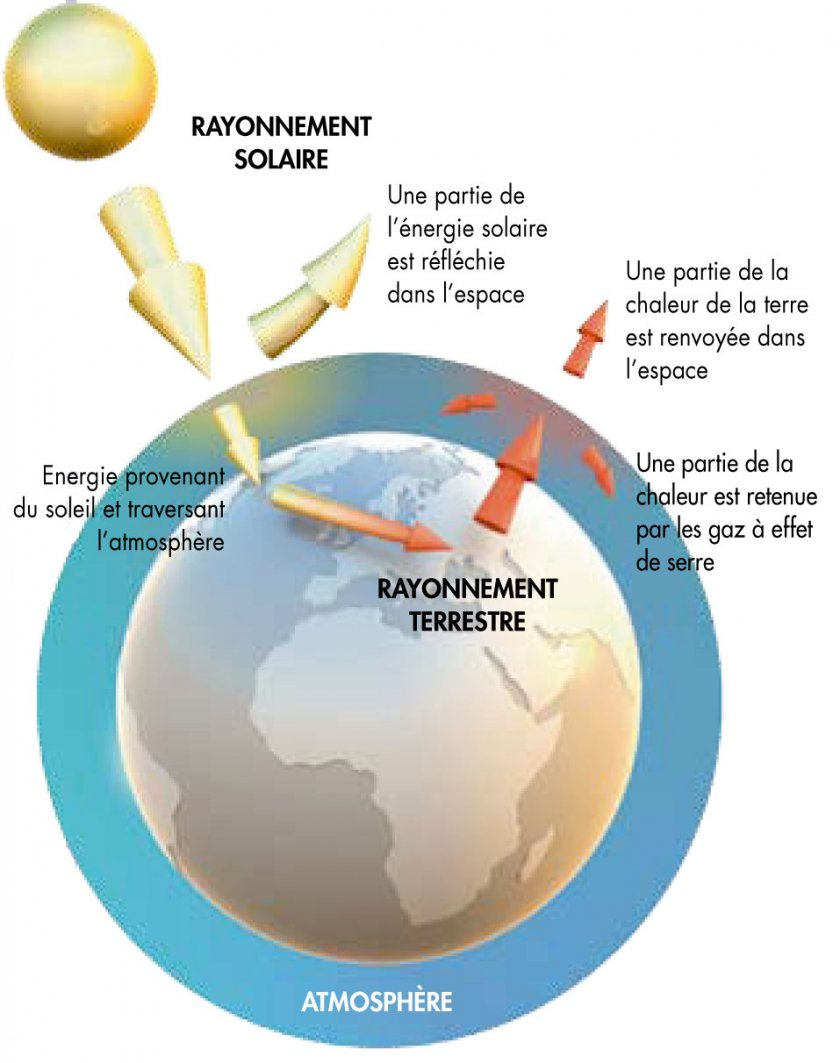
\includegraphics[scale=0.3]{fig/effet-de-serre}
    \par\end{centering}
  \caption{Schéma explicatif de l'effet de serre}
  \label{fig:effetserre}
\end{figure}


Les  gaz à  effet  de serre  peuvent  être repartis  en  deux groupes,  lesquels
existent naturellement et sont aussi produit dans l'industrie, et les outres que
sont seulement industriel.
Pour le premier groupe on a les principaux gaz à effet de serre suivant:
le vapeur d'eau, le dioxyde de carbone, le méthane,le protoxyde d'azote et l'ozone.
Pour le deuxième groupe on a des gaz fluorés comme :
les hydrochlorofluorocarbures, 
les chlorofluorocarbures, 
le tétrafluorométhane et
l'hexafluorure de soufre.

Le  tableau \ref{tab:gaz}  au dessous  démontre le  changement  de concentration
provoquer par l'homme. On peut voir que le dioxyde de carbone a une augmentation
considérable à cause de les actions anthropiques. 

\begin{table}[H]
  \caption{Comparaison entre la  concentration des gaz à effet  de serre entre les
    périodes préindustrielle e actuel }
  \begin{tabular}{ |c | c| p{3cm} | p{2.5cm} | p{2.5cm}  |}
    \hline
    Gaz à effet de serre & Formule & Concentration Préindustrielle & Concentration
    Actuelle & Durée de séjour
    (ans)  \\
    \hline 
    \hline 
    vapeur d'eau & \ce{H2O} & 3‰ & 3‰ &  (1-2 semaines) \\
    dioxyde de carbone & \ce{CO2} & 278 ppm & 387 ppm &  15 - 200 \\
    méthane & \ce{CH4} &0,7 ppm &1,7 ppm& 4 \\
    protoxyde d'azote & \ce{N2O} & 0,275 ppm &0,311 ppm &120 \\
    dichlorodifluorométhane  & \ce{CCl2F2} & 0 & 0,503 ppb & 130 \\
    chlorodifluorométhane  & \ce{CHClF2} & 0 & 0,105 ppb & 12 \\
    tétrafluorométhane & \ce{CF4} & 0& 0,070 ppb &50 000 \\
    hexafluorure de soufre & \ce{SF6} & 0 & 0,032 ppb & 3200\\
    \hline
  \end{tabular}
  \label{tab:gaz}
\end{table}

Le  tableau ci-dessous  montre le  valeur de  Potentiel de  réchauffement global
(PRG), qu'est utilisé pour prédire les impacts relatifs de différents gaz sur le
réchauffement global en se basant sur leurs propriétés radiatives.
Par définition,  le PRG du  \ce{CO2} est  toujours identique à  1 et les  autres sont
basées sur une comparaison avec le \ce{CO2}.

\begin{table}[H]
  \caption{Comparaison entre les effets des différents gaz de serre}
  \begin{center}
    \begin{tabular}{ |c | c|}
      \hline
      gaz à effet de serre &  PRG à 100 ans \\
      \hline 
      \hline 
      vapeur d'eau &  8\\
      dioxyde de carbone  & 1\\
      méthane & 23\\
      protoxyde d'azote  &310\\
      dichlorodifluorométhane  & 6 200 - 7 100\\
      chlorodifluorométhane  & 1 300 - 1 400\\
      tétrafluorométhane &6 500\\
      hexafluorure de soufre & 22 800\\
      \hline
    \end{tabular}

  \end{center}
\end{table}

Les actions qui on résulté en cette augmentation sont:

\begin{itemize}

\item L'utilisation massive de combustibles fossiles (le charbon, les produits
  pétroliers et le gaz naturel)

\item La  déforestation, parque une forêt  mature est un  réservoir important de
  carbone.

\item  Les  rejets  de  méthane non naturels  sont  dus  principalement  aux
  ruminants et aux surfaces inondées telles les rizières.

\end{itemize}



\subsection{L’impact et le danger liés au réchauffement climatique}

Le principal  impact lié  au réchauffement climatique  est l'augmentation  de la
température, dans la dernière décennie  la moyenne était $0.5^{\circ}$ plus haut
que le période entre 1961 et 1990.

Cette  augmentation de température  influence les  précipitations dans  tout le
monde,  dans quelques  lieus il  y aura  une augmentation  de  précipitation que
pourrait cause  une inondation , tandis  qu'autres lieus auront  des périodes de
sécheresse en raison d'une baisse de précipitations.

Une autre conséquence  est la diminution de la banquise,  soit dans le montagnes
(voir figure \ref{fig:kili}) soit dans les pays avec calottes polaires (Antarctique et Groenland).
Comme quelques montagnes sont la source de l'eau pour quelques civilisations, le
réchauffement climatique  aura un impact  gigantesque dans la quantité  de l'eau
disponible. Et en plus, il existe un danger de avalanche plus accentué.

\begin{figure}[H]
  \begin{centering}
    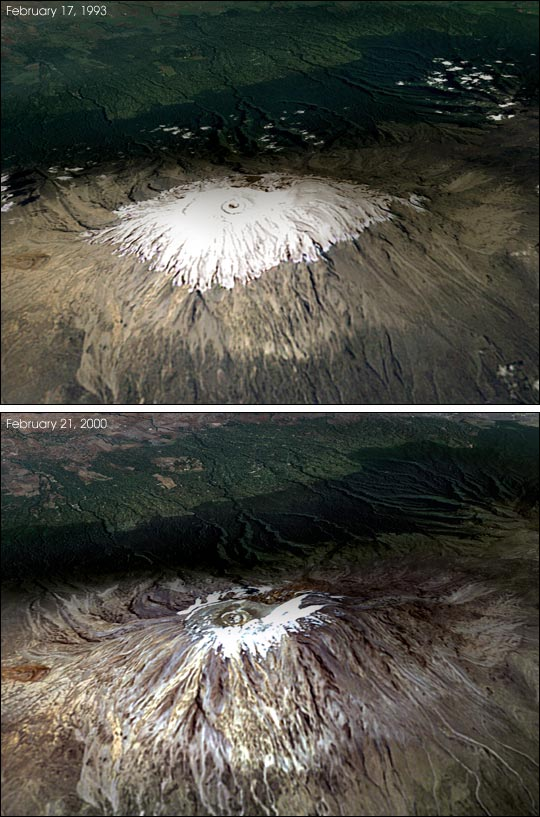
\includegraphics[scale=0.3]{fig/kili}
    \par\end{centering}
  \caption{Changement de l'accumulation des neiges au sommet du Kilimandjaro}
  \label{fig:kili}
\end{figure}


Sur  l'agriculture, les  températures  ont un  effet  sur la  date des  récoltes
agricoles, par exemple les dates de vendanges peuvent être plus avancées que le normal.

Un  changement du  climat, aura  aussi une  impact sur  le faune  et  flore, par
exemple quelques espèces à cause de  la glace fondante doivent se déplace, ainsi
comme les  du mer  qui à causse  d'une augmentation  de température de  l'eau se
déplacement pour le pôles.

D'autres danger sont:
\begin{itemize}
\item L'intensité des cyclones tropicaux va probablement augmenter.
\item Élévation  du niveau de la  mer: le niveau  a augmenté 1,8mm par  an entre
  1961 et 1993 et de 3,4 mm par an depuis 1993. Cette augmentation du niveau est
  en raison de la dilatation thermique des océans et la fonte des glaces continentales.
\end{itemize}


\subsection{Les conséquences en France}


Le réchauffement constaté en France métropolitaine au cours du $XX^e$ siècle 
est d’environ 30  \% plus grand que le réchauffement moyen  sur le globe, tandis
que  la température  moyenne annuelle  global a  augmenté de  $0,74^{\circ}C$ en
France métropolitaine la valeur est de $0,95^{\circ}C$ (voir figure \ref{fig:franceMoyenne}).
En raison de ce réchauffement, on a une augmentation des précipitations
pendant l'hiver et l'automne (entre 5 et 35 \%) et d’une baisse des précipitations
pendant l'été.

Comme prévision dans le cas plus pessimiste,  la moyenne ira augmenter environ $8,0^{\circ}C$ et
dans le cas plus optimiste $3,0^{\circ}C$.

\begin{figure}[H]
  \begin{centering}
    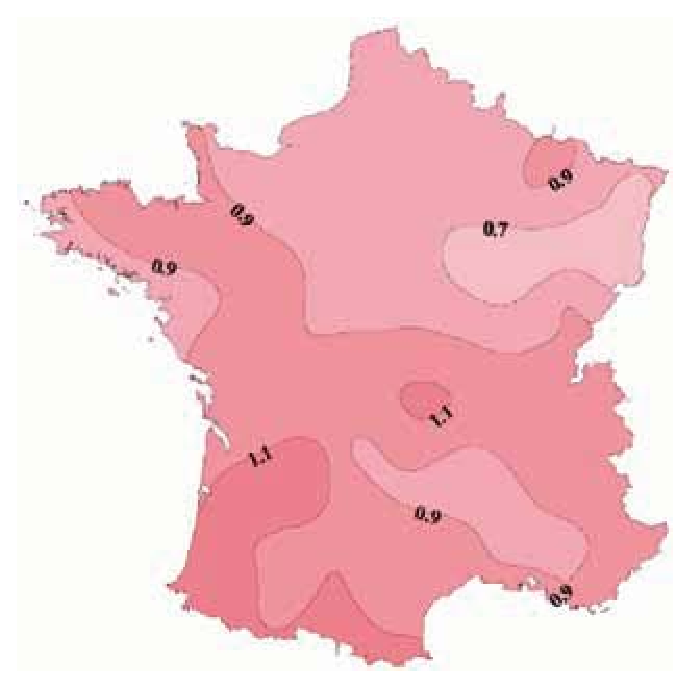
\includegraphics[scale=0.6]{fig/franceMoyenne}
    \par\end{centering}
  \caption{Augmentation de la température moyenne annuelle en France
    métropolitaine sur la période 1901-2000}
  \label{fig:franceMoyenne}
\end{figure}

Il  existera aussi  plus  de  jours avec  températures  maximales supérieures  à
$35^{\circ}C$ en  France, la  figure \ref{fig:35france} démontre  les prévisions
qui ont été  faites. Dans la situation plus pessimiste  la France souffrira plus
de cinquante jours avec de grande températures. 

\begin{figure}[H]
  \begin{centering}
    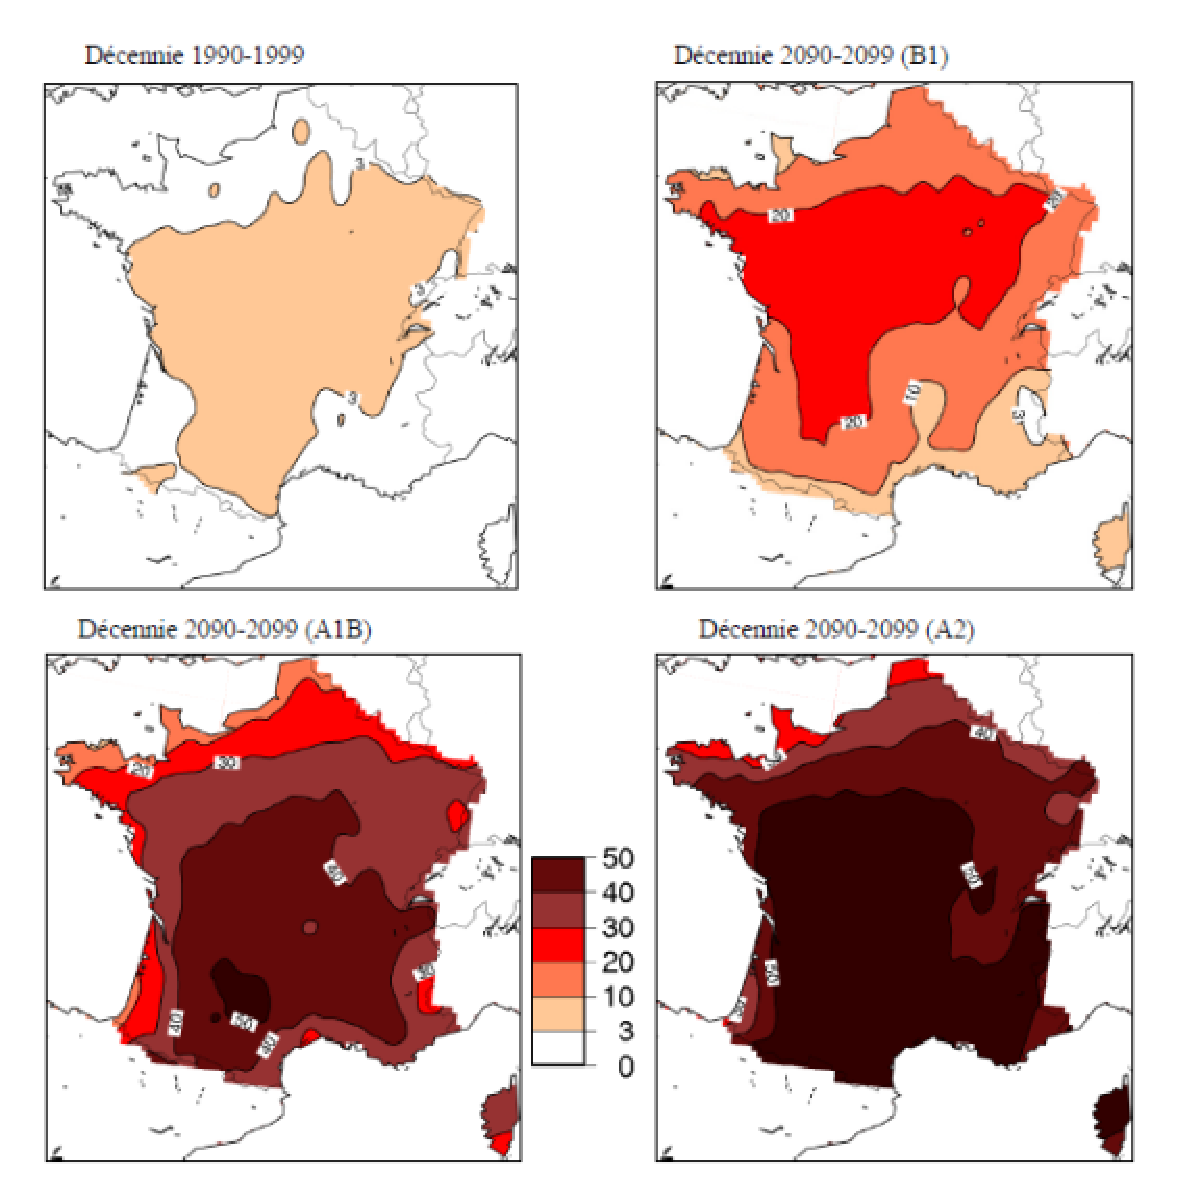
\includegraphics[scale=0.5]{fig/35france}
    \par\end{centering}
  \caption{Nombre de jours par an avec températures maximales supérieures à 35°C
    en  France :  dernière décennie  du  20 ème  siècle comparée  à la  dernière
    décennie du  21ème siècle, selon  les 3 scénarios  A2, A1B et  B1 (copyright
    Météo-France 2007)}

  \label{fig:35france}
\end{figure}


\subsubsection*{Ressource en eau}
Si l’on considère une stabilité de la demande, un déficit de 2 milliards de m3
par an  pour la satisfaction  des besoins actuels de  l’industrie, l’agriculture
(irrigation) et l’alimentation en eau potable serait observé à l’horizon 2050.

Les zones les plus vulnérables seraient les zones déjà concernées par des déficits structurels. Le coût
du déficit atteindrait 5 à 10 milliards d’euros si les volumes d’eau devaient être
complètement compensés et des traitements complémentaires mis en œuvre.

\subsubsection*{Le retrait-gonflement des sols argileux (RGA)}

Les sécheresses au été sont responsables de la majorité des sinistres liés au RGA.
En prenant compté  que les sécheresses seront intensifiés,  le coût moyen annuel
des dommages  passera d’environ 220  millions d’euros (référence sur  la période
1989-2003) à un coût entre 700 et 1 3000 millions d’euros en 2100.

\subsubsection*{Les inondations}
Avec  l'augmentation des  précipitations extrêmes  les  inondations augmenteront
aussi, donc quelques scénarios ont été créer pour quelques bassins versants.
Le tableau ci-dessous démontre que les  évolutions de dommages sont grand sur la
Meuse et  l'Orb, cela veut dire  que la probabilité  d'inondation ira augmenter
considérablement. 


\begin{table}[H]
  \begin{center}
    \caption{Variation du début de pointe retenues sur les bassins versants d’illustration}
    \begin{tabular}{|c|c|c|c|}
      \hline
      & Hypothèse basse &Hypothèse moyenne &Hypothèse haute\\
      \hline
      Loire & +5 \% & + 10 \% & +20\%\\
      Seine & - 10 \% &+ 10 \% & - \\ 
      Rhône & 5\% & 10 \% & +20\%\\
      Meuse & 10\%& 10\%& +10\%\\
      Orb &10\% & 25\% & +50\% \\
      \hline
    \end{tabular}
  \end{center}
\end{table}

\subsubsection*{Impact sur la couverture neigeuse}
Comme la  couverture neigeuse des massifs  montagneux français sont  liées a bas
températures,  le   réchauffement  climatique  tend  à  diminuer   la  durée  de
l’enneigement et l’épaisseur  du manteau neigeux. De même  façon il existera des
modifications  des  régimes  hydrologiques  des  rivières  de  montagne,  de  la
végétation à haute altitude et de l’enneigement des stations de sport d’hiver. 


\subsubsection*{Impact sur l’agriculture}
Dans une côté, le sud de la France devraient apparaître des effets négatifs, qui
peuvent  prendre une  grande  ampleur dans  le  cas de  sécheresses répétées  et
persistante. Dans autre côté, des effets plutôt positifs sont à attendre dans le
nord parce que les mauvaises herbes seront les plus impactées.

Par exemple, le blé aura une augmentation des rendements, pendant que le maïs en 2100
à une perte pouvant atteindre près de 113 millions d’euros par an.

Autre  grand  impact  sur  l'agriculture  sera l'augmentation  des  périodes  de
canicule, par exemple,  un canicule comme l'un de  2003 pourrait représenter, en
2100,  un coût  allant jusqu’à  plus de  300 millions  d’euros par  an  pour une
culture comme le blé.  

Pour la viticulture, il ne sera pas
possible dans ces conditions de produire autant de vins de haute qualité qu’au-
jourd’hui. En plus, Il existera des pertes de rendement considérables (jusque - 26 \%).

\subsubsection*{Impact sur la santé }
La canicule de 2003 en France a provoqué une surmortalité observée de 14 800
personnes entre le 1er et le 20 août.  Et est estimé que la valeur perdue par la
societé française est environ 500 millions d’euros.
Comme un mécanisme d'alerte aux ondes de chaleur, le Plan national canicule
(PNC) a été mis en place.Le coût  pour la préparation du système plus le coût de
fonctionnement est d'environ 740 000 euros. 

\subsubsection*{Impact énergétiques}
La consommation énergétique  en régions de climat frais  ira, peut-être diminuer
en raison  d'une économie  en chauffage, cependant  augmenterait dans  les zones
méridionales en raison d'une forte dépense en climatisation.

Les baisses de précipitations modélisées dans les principaux bassins versants
aménagés en unités hydro-électriques laissent envisager une baisse moyenne de
l’ordre de 15 \% du potentiel productible.


\section{La position de la société française}
\subsection{Les écologistes}

Les ONG écologistes estiment toujours que les politiques européennes ne vont pas
assez loin,  cela veut dire que  les efforts font pour  ramener le réchauffement
climatique à un niveau moins intense sont insuffisantes, par exemple l' objectif 
de réduction de 20\% plutôt que 30\% est inacceptable .
  Ainsi, les ONG
(CAN\footnote{Le  réseau  action climat  Europe  (CAN-E)  est  reconnu comme  le
  premier réseau européen dans le domaine du climat et des énergies. CAN-E lutte
  contre le  changement climatique et  promeut les énergies renouvelables  et la
  politique environnementale européenne.}
Europe, Friends  of Earth\footnote{Les Amis de  la Terre (Friends  of Earth) est
  une  organisation non  gouvernementale (ONG)  de protection  de l'Homme  et de
  l'environnement    créée   en    1969,   et    présente   dans    76   pays.},
Greenpeace\footnote{ Le  greenpeace est une organisation  non gouvernementale de
  protection de l'environnement présente dans plus de quarante pays à travers le
  monde.}  et le  WWF\footnote{Le World  Wide Fund  for Nature  est  la première
  organisation mondiale de protection de  la nature.}) ont exigé une révision en
profondeur  du  PECC  (Programme  européen  sur le  changement  climatique),  et
l'établissement d'objectifs et de politiques plus ambitieux.  



À cause de cette faible ambition, les ONG supportent que la révolution énergétique
européenne est une ``rêve encore lointain'' et que les propositions
dans le domaine de l'énergie ``ne  sont pas convaincantes et pourraient avoir des
conséquences  négatives,  notamment en  ce  qui  concerne  les biocarburants  et
l'énergie nucléaire.''~\cite{ONG}


\subsection{La société en général} 

Selon des sondages environ 84\% des Français croient à la réalité du réchauffement
climatique et  parmi ces  personnes  96\% disent que  les activités
humaines ont intensifié le phénomène.
Toutefois, parmi les 84\% seulement 40\% y croient "tout à fait", pendant que les autres déclarent "plutôt" y
croire (44\%). 

Cependant, seulement 31\% des Français sont convaincus que le réchauffement climatique est
scientifiquement prouvé.

De plus, la plupart des Français considèrent que les conséquences des activités humaines
sur le réchauffement climatique sont minorées (49\%) ou exagérées (33\%). 
Ainsi, ces résultats démontrent qu'il existe des doutes sur la crédibilité des scientifiques sur le
sujet. 

Par ailleurs, seulement 56\% des Français pensent que de mesures pour résoudre le
problème au niveau mondial seront prises dans  les prochaines années  pour freiner le réchauffement  climatique.

\subsection{Les entreprises}

Les entreprises européens jugent que la politique  de  lutte  contre  le
changement climatique de l'UE les nuisent, et alors affect sa position concurrentielle dans l'économie
mondiale. Ils  ont, plusieurs  fois , critiqué  la stratégie  "unilatérale" (une
solution seulement européenne) en
soulignant la nécessité de solutions globales.

Par  exemple, en  2009  plusieurs fédérations  professionnelles  comme UNICE  et
Eurochambres, ainsi que le Conseil  européen de l'industrie chimique (CEFIC) ont
critiqué le caractère  unilatéral des objectifs de réduction  d'émissions de CO2
en  disant que  les  objectifs de  réduction  étions trop  élevés,  et comme  il
existait des grand  pays pollueurs qui ne feraient pas  cette réduction, cela
affaiblirait la compétitivité de l'Europe dans le monde sans avoir de véritables effets sur la
protection de l'environnement.

D'autre part, l'industrie a peur d'une hausse du prix d'énergie renouvelable, et
cela hausserai  les prix de  toutes les choses.  Pour que cette  prix n'augmente
pas, une offert d'énergie nucléaire doit être intensifié.

% \subsection{Les économistes} 

\section{La position de la France dans le monde}

\subsection{L’avis du gouvernement  Français}

Le gouvernement français participe activement dans les sommets sur la situation du réchauffement climatique où sont fixes los objectifs de réduction des émissions à moyen terme conformément aux recommandations scientifiques. 

D'une part, la France a créé l’Agence française de développement (AFD) pour développer le soutien budgétaire en faveur de pays mettant en œuvre projets d’intégration du climat dans leur stratégie de déploiement. L’AFD a ainsi déjà soutenu, en coopération avec d’autres financeurs internationaux, des pays comme l’Indonésie, le Mexique, le Vietnam et l’île Maurice. Ce plan a eu au total 1,7 milliard de dollars d’investissement depuis 2008.

À ce sujet, la France met en œuvre un effort supplémentaire de 1,26 milliard d’euros sur la période 2010-2012 au titre de son engagement pris à Copenhague de financement précoce de sorte que le 20 \% de sa contribution soit destiné à la forêt.

D’autre part, le Fonds Français pour l'Environnement Mondial (FFEM) est un fonds public bilatéral créé par le gouvernement français en 1994 pour accompagner les pays en développement à mettre en œuvre des stratégies et des projets innovants conciliant préservation de l’environnement et développement économique et social. En partenariat avec des autres acteurs publics, le FFEM subventionne des opérations innovantes dans les principaux domaines de l’environnement mondial comme le changement climatique, biodiversité, déforestation et désertification.

D’ailleurs, la France soutient le développement de partenariats concrets en complément des négociations, et promeut à ce titre l’initiative pour développer l'accès aux énergies propres dans les pays les plus vulnérables aux changements climatiques. Un exemple concret est le projet « Paris-Nairobi », lancée avec le Kenya le 21 avril dernier. En outre, la présidence française du G20\footnote{Le Groupe des 20 est un groupe de 19 pays plus l'Union européenne dont les ministres, les chefs des banques centrales et les chefs d'États se réunissent régulièrement pour favoriser la concertation internationale.} s’est particulièrement impliquée dans la promotion du développement des infrastructures en Afrique, notamment dans le domaine de l’énergie. 

Par rapport aux événements récents, la France consent l'accord de Durban (conformément aux décisions prises à Cancun) qui permettre de renforcer l’ambition du régime international de lutte contre le changement climatique. En conformité avec l’Union européenne, elle continuera à assumer toutes ses responsabilités et à rester force de proposition principale contre le changement climatique. 

Cette aide offerte par la France se concrétisera comme suit:
\begin{enumerate}
\item Par le canal multilatéral, avec une participation à la reconstitution du Fonds pour L'environnement Mondial (FEM) et une contribution au Fonds pour les technologies propres de la Banque mondiale.
\item Par le canal bilatéral, avec la reconstitution du FFEM et les interventions de l’AFD.
\end{enumerate}

\subsection{Loi et taxes}

\subsubsection{La taxe carbone}

C’est  un projet  de  loi  de contribution  au  climat et  l’énergie  qui a  été
abandonné en  2010 par le  gouvernement français car  à cette époque ce  type de
projet devait être Européen et pas uniquement français. 


Ce projet  connu comme la «Taxe carbone»  est de retour pour  l’année 2012 comme
une taxe exceptionnelle  sur le CO2 orientée aux gros  pollueurs, cela veut dire
de taxer les 400 entreprises françaises  les plus émettrices de CO2 (à partir de
60 000 tonnes de rejets par an). 


Cette taxe exceptionnelle pourrait engendrer une recette de 220 millions d’Euros
pour le  gouvernement et sera  inscrite dans le  projet de loi de  finances pour
cette année. Les  secteurs d’activités les plus concernés  par cette taxe seront
la chimie, l’agroalimentaire, l’électricité et les grandes chaufferies. 


Néanmoins, le Groupe des Fédérations Industrielles (GFI) estime que cette taxe va nuire grandement à leur compétitivité à cause du coût de 150 millions d’Euros pour les industries françaises. De plus, le GFI affirme que l’assiette du chiffre d’affaire n’est pas adaptée dans l’économie moderne. Il propose au gouvernement d’instaurer à la place un système d’enchère pour l’acquisition de quotas de CO2 supplémentaires en 2012.
Par  ailleurs, Eva Joly,  la candidate  du parti  politique Europe  Écologie Les
Verts  propose  une  taxe  sur  les  énergies  non  renouvelables  (fossiles  et
nucléaires)  qui selon  elle  rapporterait  12 milliards  d’Euros  avec la  taxe
carbone et  qui pourrait permettre la  mise en place  de « chèques verts  » pour
inciter les citoyens et les entreprises à changer leurs habitudes.


\subsubsection[La loi sur l’eau et les milieux aquatiques (LEMA)]{La loi sur l’eau et les milieux aquatiques (LEMA) du 30 décembre 2006}

Cette loi propose la mise en place de mesures contre les pollutions diffuses dans les secteurs sensibles comme les zones d’alimentation des captages, les zones humides d’intérêt particulier et d’érosion diffuse.
Elle donne les moyens de contrôle de vente des produits polluants. La taxe globale associé a ce type d’activité sur les produits phytosanitaires est transformée en une redevance au profit des agences de l’eau prenant en compte toxicité de ces produits.

\subsubsection{Taxe sur des émissions des secteurs maritimes et des transports aériens}

La France évalue comme option de financement innovant une taxe sur les émissions
des secteurs  maritimes et des  transports aériens. Ces  financements innovants,
portés par  la présidence française  dans le cadre  du G20 joueront un  rôle clé
pour  atteindre ces  objectifs, cela  veut dire  de mobiliser  100  milliards de
dollars chaque année et ce à l’horizon 2020 notamment pour le nouveau Fonds vert
pour le climat.


Aujourd'hui ni le  secteur aérien ni le transport  maritime, qui représentent un
pourcentage importante des  émissions globales de gaz à effet  de serre, ne sont
pas soumis  à des contraintes de  réduction de ses émissions.  Mais, d’être fixé
cette taxe pourrait restreignit les activités polluantes dans ces industries.


\subsection{Les traités internationaux}

\subsubsection[Le protocole de Kyoto]{Le protocole de Kyoto: 3ème Conférence des Nations Unies sur les changements climatiques  (01/12/1997)}

Le protocole de  Kyoto, signé en 1997  mais en vigueur depuis 2005,  a prévu des
engagements de réduction des émissions de la part des 38 pays industrialisés qui
se sont  engagés à réduire  les émissions de  gaz à effet  de serre de  5,2\% en
moyenne  au 2012  (année  où le  protocole  expire), par  rapport  au niveau  de
1990. La  France a signé  le protocole  de Kyoto en  1998, elle s’est  engagée à
réduire  ses  émissions  de  gaz  à  effet de  serre  selon  les  résultats  des
négociations.


Ils  se  sont engagés  à  réduire  leurs émissions  par  rapport  à  1990 :  les
Etats-Unis de  7\%, l’Union  européenne de 8\%,  le Japon  et le Canada  de 6\%,
tandis que des  pays comme l’Australie, l’Islande se sont  engagés à contenir la
progression de leurs émissions.


Malgré  les accords conclus  à Kyoto  et sous  la pression  d'un groupe  de pays
conduits  par les  Etats-Unis, des  mécanismes  de flexibilité  sont créés  pour
permetre aux pays de remplir leurs obligations non pas en limitant ses émissions
mais en finançant des réductions à l'étranger. 


En ce qui concerne  a le fait de refuser de participer  à ce protocole, certains
pays estiment  que les mesures accordés  sont trop strictes, un  exemple de cela
est lorsque un pays ne respecte pas son engagement, il doit verser de l’argent à
l’Organisation des Nations unies (ONU) qui  le reverse à des pays qui produisent
peu de gaz à effet de serre et qui sont souvent plus pauvres.


En mars  2001 les Etats-Unis, pays  où les émissions représentant  en effet 25\%
des   émissions   mondiales,   ont   refusé   de  ratifier   le   protocole   de
Kyoto. Cependant,  Les autres pays  industrialisés ont décidé de  poursuivre les
négociations et d'appliquer ce protocole.


En décembre  2011 Canada  a décidé  de sortir du  protocole car  le gouvernement
estime qu’il  ne pourra  jamais respecter ses  engagements, et qu’il  devra trop
payer.


\subsubsection[Le sommet à Copenhague]{Le sommet à Copenhague : Le sommet des Nations unies sur les changements climatiques (7/12/2009)}

D’abord, les pays développés ont  pris l'engagement collectif de financer sur la
période 2010-2012,  à titre de  «démarrage précoce» («fast start»),  des actions
dans  les pays  en développement  en  faveur de  la lutte  contre le  changement
climatique. Cet engagement a été décidé pour un montant global de 30 milliards
de dollars ce  qui représente pour l'Union européenne et  ses Etats membres, sur
la période de trois ans, un effort de 7,2 milliards d'euros et particulièrement
1,26 milliard d'euros pour la France. 

Pourtant, il n’y a pas eu un  consensus entre les délégués des 193 pays réunis à
Copenhague,  cela a  terminé par  l’adoption  d’un texte  mis au  point par  les
Etats-Unis et quatre pays émergents, la Chine, le Brésil, l'Inde et l'Afrique du
Sud. Ce texte souligne la nécessité de limiter le réchauffement planétaire à 2°C
par rapport à  l’ère pré-industrielle mais ne comporte  aucun engagement chiffré
de réduction des émissions de gaz à effet de serre. 


\subsubsection[L’accord au sommet de Cancun sur le climat]{L’accord au sommet de Cancun sur le climat (10/12/2010)}

Dans le  cadre de cette  conférence s’est adopté  à la quasi unanimité  (sauf la
Bolivie),  un texte mettant  en place  une série  de mécanismes  financiers pour
lutter  contre le  réchauffement  climatique et  promouvoir  l'adaptation à  ses
effets. C’est  à dire  la création  d’un fonds vert  pour soutenir  les projets,
programmes et politiques d'adaptation des pays en développement. 


En effet, l'accord de Cancun ne repose que sur des mécanismes non-contraignants,
confirmant  les les  décisions  prises à  Copenhague,  et ne  prévoit rien  pour
prolonger le protocole  de Kyoto au delà  de 2012. De plus, il  est consideré la
mise en place  du mécanisme REDD (Ressources pour  le développement durable) qui
consiste à  rémunérer financièrement les populations locales  impliquées dans la
gestion des forêts. 


Par  ailleurs, Les  décisions  de Cancun  réaffirment  et amplifient  l’ambition
collective  de  réduction des  émissions  qui avait  été  celle  de l’accord  de
Copenhague,  ces  décisions comportent  aussi  des  mesures  concrètes dans  les
domaines  technologiques,  le  Fonds  vers,  du mécanisme  de  lutte  contre  la
déforestation (REDD), ainsi  que le développement propre aux  projets de capture
et de stockage du carbone.


En dernier lieu,  selon les acquis de  Copenhague et de Cancún, le  but des pays
forestiers est d’abord  élaborer des stratégies nationales pour  mettre en place
des  systèmes  de  suivi de  l’état  des  forêts  pour renforcer  les  capacités
institutionnelles et la  expérience dans les projets pilotes  à l’échelle locale
et régionale.


\subsubsection[La conférence annuelle des Nations-Unies sur le climat de Durban]{La conférence annuelle des Nations-Unies sur le climat de Durban (11/12/2011)}

Dans  un premier  temps l’'un  des défis  de Durban  était de  mettre  en oeuvre
certaines  des  décisions  prises  à  Cancun,  notamment  sur  le  sujet  de  la
transparence  et  de la  vérification  possible  des  actions de  réduction  des
différents pays. 


Un des sujets abordés a été le Fonds vert pour aider les pays en développement à
faire face au changement climatique.  Ce Fonds doit acheminer des financements à
partir de 2013 pour monter en puissance jusqu'en 2020, date à partir de laquelle
les  pays industrialisés  ont promis  de verser  chaque année  100  milliards de
dollars.


D’autre  part, l'accord  prévoit  par ailleurs  la  mise en  place d'un  travail
préparatoire pour éventuellement faire entrer l'agriculture, à l'origine de 15\%
des émissions de gaz à effet de serre. 


Pourtant, le  résultat c’est un  document habilitant, qui reconnaît  l'écart des
émissions, confirme l'objectif à long terme, et encourage le multilatéralisme.


De plus, la décision de Durban prévoit  une deuxième période dont la durée (5 ou
8 ans) doit encore  être débattue. Mais en l'absence du Canada,  de la Russie et
du  Japon, qui  ont refusé  de renouveler  l'exercice, ces  nouveaux engagements
contraignants  ne s'appliqueront qu'à  environ 15\%  des émissions  mondiales en
raison du volume impliqué dans les pays participants.


Finalemente, au  futur, la possibilité  d'une seconde période  d'engagements sur
Kyoto serait  discuté et signé en  2015 pour une  entrée en vigueur à  partir de
2020. 


\section{Analyse des solutions proposés par chaque partie}

\subsection{Présentation des solutions}

Pendant les dernières  années plusieurs conférences entre pays  ont été réalises
pour  développer  les  solutions   plus  efficaces  pour  résoudre  le  problème
climatique. L’un de plus importants est la réduction des émissions et les seuils
de  précaution   scientifiques  pour  limiter  le   réchauffement  climatique  à
1,5°C. Cela impliquerait que les  pays industrialisés amorcent des réductions de
25\% à 40\% d'ici à 2020. 


Les  pays  développés  comme  ceux  de  l’UE,  la  Norvège,  l'Australie  et  la
Nouvelle-Zélande ont  accepté de participer à une  deuxième période d'engagement
du Protocole  de Kyoto qui débuterait  au 1er Janvier 2013  et s'étendre jusqu'à
2017 ou 2020 (période pas encore défini). C’est important de noter que l'étendue
de la participation du Japon, la Russie  et le Canada dans le Protocole de Kyoto
phase  II reste incertaine,  même si  ils ont  dit clairement  non avant  la COP
(Conférence des parties).


Par  ailleurs,  les  pays  ont  convenu  de travailler  sur  un  nouveau  traité
climatique international  qui inclurait pour  la première fois les  deux groupes
des  pays  (ceux  développés  et  ceux en  développement).  Ils  décideront  des
modalités de ce traité en 2015 et sa  mise en œuvre à partir de 2020. Ainsi, les
grands émetteurs comme la Chine, l'Inde et Etats-Unis auront engagements légales
d'émissions après 2020. 


Ainsi, une  des principales  solutions proposées, le  Fonds vert pour  le climat
(GCF  en  anglais)  de  100  milliards  de  dollars  (en  2020)  est  maintenant
opérationnel  et  aura sa  première  réunion  en Suisse  avec  la  Corée du  Sud
fournissant démarrage financement pour le fonds. Bien que son lancement a été un
succès  notable, il  existe le  défaut  de fournir  des signaux  clairs sur  les
méthodes de financement à long terme  pour soutenir les pays en développement ce
que peut être décevant. 


Dernièrement, l’année prochaine se réalisera la COP 18 à Qatar où les sujets sur
les  rapports  techniques  à  utiliser  et  la base  pour  la  détermination  de
financement à long terme seront abordés.


\subsection{Comparaison des solutions et son impact dans la société}

Les solutions proposés ont deux impacts différents par rapport aux types de pays, les émergents et les développés.

D’une part, selon l'Agence Internationale  d'énergie, la Chine va conforter dans
les  20  prochaines  années   sa  position  de  premier  consommateur  d'énergie
mondial. Ses émissions per capita  atteindront celles des pays très polluants en
2035. Quant au Brésil, il vient de  réformer son code forestier ce qui permet la
destruction massive de son précieux écosystème. 


D’autre part, l'immensité  du défi, combinée à la crise  de la dette européenne,
prive la planète de leaders à la  mesure de l'enjeu. Tandis que l'Inde, la Chine
et les  Etats-Unis concourent à torpiller  le processus, l'Europe,  minée par la
crise de la dette, se divise. 


Enfin, le  Fonds vert, principal  acquis de la  négociation à Cancun,  destiné à
soutenir  les  pays  vulnérables   aux  conséquences  du  réchauffement,  et  au
financement   d'une  transition   énergétique  soutenable   dans  les   pays  en
développement, ce Fonds, qui devait être abondé de 30 milliards de dollars entre
2010 et  2012, puis  de 100 milliards  de dollars  par an à  partir de  2020, ne
récolte que  quelques dizaines  de millions  de dollars pour  le moment.  Ce qui
n’arrive pas  aux objectifs  attendus et  qui démontre qu’il  manque un  un long
chemin pour développer et aller négocier.



% \section{L’avis du gouvernement}
% \subsection{Les politiciens}
% \subsection{Les lois et taxes}
% \subsection{Les traités internationaux}


% \section{Analyse des solutions proposés par chaque partie}
% \subsection{Présentation des solutions}
% \subsection{Comparaison des solutions et son impact dans la société}


\section*{Conclusion}

% ******************************************************
% REFERENCIAS BIBLIOGRÁFICAS
% ******************************************************
% \section{Referências}
\bibliographystyle{plain}
\begin{small}
  \bibliography{Bibliographie}
\end{small}
\section*{}

\end{document}